\documentclass{beamer}


% ---
% PACOTES
% ---

% ---
% Pacotes fundamentais 
% ---
\usepackage{times}         % Usa a fonte Latin Modern
\usepackage[T1]{fontenc}      % Selecao de codigos de fonte.
\usepackage[utf8]{inputenc}      % Codificacao do documento (conversão automática dos acentos)
\usepackage{indentfirst}      % Indenta o primeiro parágrafo de cada seção.
\usepackage{nomencl}          % Lista de simbolos
\usepackage{color}            % Controle das cores
\usepackage{graphicx}         % Inclusão de gráficos
\usepackage{microtype}        % para melhorias de justificação
\usepackage{ordinalpt}
% ---
% ---
% Pacotes adicionais, usados apenas no âmbito do Modelo Canônico do abnteX2
% ---
\usepackage{lipsum}           % para geração de dummy text
% ---
      
% ---
% Pacotes de citações
% ---
\usepackage[brazilian,hyperpageref]{backref}  % Paginas com as citações na bibl
\usepackage[alf]{abntex2cite} % Citações padrão ABNT
% ---

% ---
% Configurações do pacote backref
% Usado sem a opção hyperpageref de backref
\renewcommand{\backrefpagesname}{Citado na(s) página(s):~}
% Texto padrão antes do número das páginas
\renewcommand{\backref}{}
% Define os textos da citação
\renewcommand*{\backrefalt}[4]{
   \ifcase #1 %
      Nenhuma citação no texto.%
   \or
      Citado na página #2.%
   \else
      Citado #1 vezes nas páginas #2.%
   \fi}%
% ---
\usetheme{Berlin}

% --- Informações de dados para CAPA e FOLHA DE ROSTO ---
\title{Análise de conteúdo numa perspectiva de Bardin}

\author{João Henrique da Silva\\
--
Prof. Dr. Carlos Alberto de Oliveira Magalhães Júnior}
\institute{UEM DCI PROFCIAMB}
\logo{

\includegraphics[width=1cm]{logo.png}

\includegraphics[width=1cm]{uem.png}
}

%\local{Brasil}
\date{Junho - 2022}
% ---

% ---
% Configurações de aparência do PDF final

% alterando o aspecto da cor azul
\definecolor{blue}{RGB}{41,5,195}

% informações do PDF
\makeatletter
\hypersetup{
      %pagebackref=true,
      pdftitle={\@title}, 
      pdfauthor={\@author},
      pdfsubject={},
      pdfcreator={},
      pdfkeywords={abnt}{latex}{abntex}{abntex2}{atigo científico}, 
      colorlinks=true,           % false: boxed links; true: colored links
      linkcolor=blue,            % color of internal links
      citecolor=blue,            % color of links to bibliography
      filecolor=magenta,            % color of file links
      urlcolor=blue,
      bookmarksdepth=4
}
\makeatother
% --- 

% ---
% compila o indice
% ---
\makeindex
% ---



% --- 
% Espaçamentos entre linhas e parágrafos 
% --- 

% O tamanho do parágrafo é dado por:
\setlength{\parindent}{1.3cm}

% Controle do espaçamento entre um parágrafo e outro:
\setlength{\parskip}{0.2cm}  % tente também \onelineskip

% Espaçamento simples
\linespread{1.3}


%\usetheme{lucid}
\begin{document}
    \frame {
        \titlepage
    }

    \frame {
        \frametitle{Análise de Conteúdo - AC}
        \framesubtitle{A contribuição de Laurence Bardin}
	\begin{itemize}
		\item A análise qualitativa de fontes diversas, textos, questionários, notícias e livros requer ferramentas heurísticas 
		\item Metodologia quali; quali-quanti
		\item Função Heurística: visa organizar a inferência de informações
        \item Função de administração de provas: arca com o ônus probatório colocado pelas hipóteses levantadas
	\end{itemize}
    }

    \frame{
        \frametitle{Análise de Conteúdo - AC}
        \framesubtitle{Histórico da análise de conteúdo - 1}
        \begin{itemize}
            \item A metodologia hermenêutica que analisa a exegese \cite[p.289]{bardin_epistemologia}
            \item Primeira Guerra - Análise das publicações da imprensa e Governos
            \item Segunda Guerra - Busca de propaganda subversiva e policiamento ideológico
            \item Abordagem quali-quanti emerge na década de 50 com o foco na descrição sistemática e objetiva
        \end{itemize}
    }

    \frame{
        \frametitle{Análise de Conteúdo - AC}
        \framesubtitle{Histórico da análise de conteúdo - 2}
        \begin{itemize}
            \item Questionamentos acerca da eficácia do modelo; excesso de rigor e objetividade consolidaram a abordagem quali-quanti
            \item Métodos estatísticos para determinar as frequências e coocorrências permitem inferências justificadas e deduções lógicas
            \item Procedimentos que convergem com a atividade de Inteligência OSINT - Open source Inteligence e DOMEX - document and media exploitation \cite[1-25]{FM_2-0}
        \end{itemize}

    }
    \frame{
        \begin{figure}
          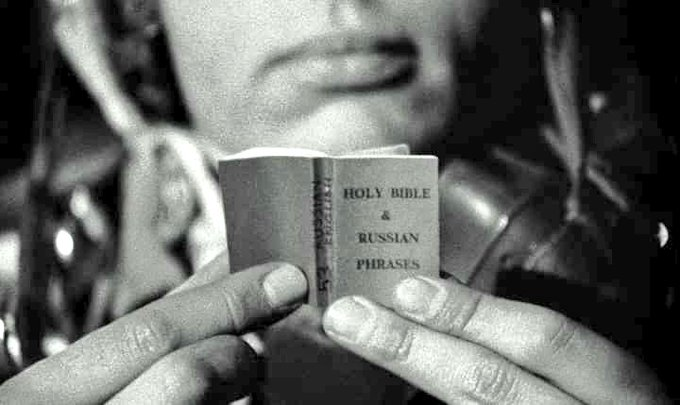
\includegraphics[width=80mm,scale=1]{russia.jpeg}
        \end{figure}
        Cena do Filme Dr. Strangelove or: How I Learned to Stop Worrying and Love the Bomb - 1964 do diretor Stanley Kubrick.
    }

    \frame{
        \frametitle{Análise de Conteúdo - AC}
        \framesubtitle{Alguns aspectos da análise de conteúdo}
        \begin{itemize}
            \item Metodologias do pesquisador e do espião; identificar o que está implícito no corpus
            \item Pesquisador deve controlar sua própria perspectiva e subjetividade na busca da sistematização, objetividade e generalização
            \item Exemplos de análise de frequências e coocorências \cite{Python_NLTK_freqs}
        \end{itemize}
    }

    \frame{
        \frametitle{Análise de Conteúdo - AC}
        \framesubtitle{frequências no corpus}
        \begin{figure}
          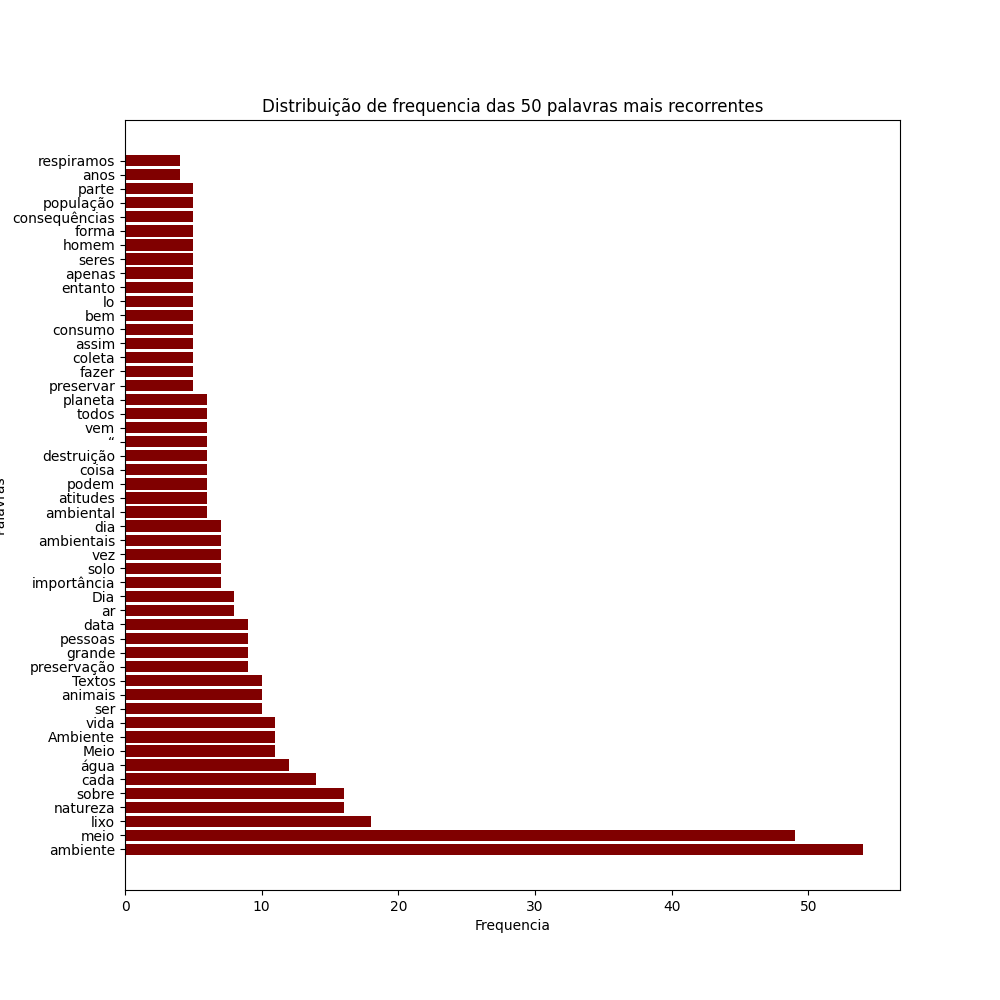
\includegraphics[scale=0.25]{Figure_1_dist_pal.png}
        \end{figure}
    }

    \frame{
        \frametitle{Análise de Conteúdo - AC}
        \framesubtitle{coocorências no corpus}
        \begin{table}
        \tiny
        \centering
        \caption{Python -Função corpus collocation list}
        \begin{tabular}{lll}
            & meio & ambiente \\
            & Meio & Ambiente \\
            & Textos & sobre \\
            & sobre & meio \\
            & Nações & Unidas \\
            & sua & parte \\
            & coleta & seletiva \\
            & uma & grande \\
            & Dia & Mundial \\
            & seres & vivos \\
        \end{tabular}
        \begin{tabular}{lll}
            & problemas & ambientais \\
            & 113 & países \\
            & 250 & organizações \\
            & impactos & negativos \\
            & matéria & prima \\
            & reuniu & 113 \\
            & cada & pessoa \\
            & das & Nações \\
            & jogar & lixo \\
            & que & respiramos 
        \end{tabular}
        \end{table}
    }

    \frame{
        \frametitle{Análise de Conteúdo - AC}
        \framesubtitle{Etapas para o desenvolvimento da AC}
        \begin{itemize}
            \item Pré-análise via leitura flutuante e formulação de hipóteses
            \item Codificação dos dados e categorização; unidades de registro; temas ou frases recorrentes
            \item Unidades de contexto; espalhamento usado pela linguagem usada para descrever os fenômenos
            \item Inferências e validação das hipóteses; interpretação
        \end{itemize}
    }

    \frame{
        \frametitle{Análise de Conteúdo - AC}
        \framesubtitle{Critérios para o desenvolvimento da AC}
        \begin{itemize}
            \item Exaustividade; analisar todos os elementos do corpus
            \item Representatividade; amostragem rigorosa
            \item Homogeneidade; padronização dos documentos
            \item Pertinência; adequação das fontes de informação
        \end{itemize}
    }

    \frame{
        \frametitle{Análise de Conteúdo - AC}
        \framesubtitle{Unidades de significação}
        \begin{itemize}
            \item Unidades de registro; segmento de conteúdo organizado semanticamente; palavras-chave que permitem a contagem frequencial
            \item Unidades de contexto; compreensão da significação presente nas unidades de registro
            \item Atribuição de pesos durante a enumeração das frequências
        \end{itemize}
    }

    \frame{
        \frametitle{Análise de Conteúdo - AC}
        \framesubtitle{Desmontagem dos dados e construção das categorias}
        \begin{itemize}
            \item Exclusão mútua; unidade de registro sópode ser classificada em uma categoria
            \item Homogeneidade na construção das categorias
            \item Pertinência das informações dentro de cada categoria
            \item Objetividade e fidelidade; definição de índices claros para a inserção das unidades de registro em uma dada categoria
            \item Produtividade; categoria precisa ter capacidade explicativa para validar a inferência dos dados
        \end{itemize}
    }


\bibliography{interdisciplinaridade}
\end{document}



